\section{Node.js}
Sirve para algunas cosas.
%%%%%%%%%%%%%%%%%%%%%%%%%%%%%%%%%%%%%%%%%%%%%%%%%%%%%%%%%%%%%%%%%%%%%%%%%%%%%%%%%%%%%%%%%%%%%%%%
\section{Historia de JavaScript}
\begin{enumerate}
    \item Fue inventado por Brendan Eich en 10 días, tiene similitudes con java pero solo fue una estrategia de java.
    \item Fue innorvador tener la capacidad de un  browser, JavaScript se llamaba moca, liveScript, JavaScript.
    \item El proposito de esto fue ofrecer una experiencia interactiva, surgen los juegos.
    \item Se requería plug-ins para JavaScript para usar calculadoras en línea por ejemplo.
    \item Surge una gran infección de viruses que atentaba en contra de industria, era muy vulnerable a la seguridad y el punto de entrada de estos viruses por medio de los plug-ins.
    \item Entonces como medida de seguridad se desarrollan nuevos browsers que aseguran que el código de las páginas web cambiara algo de tus archivos locales, pero se volvió un asunto que era incompatible todo con todo.
    \item Como solución a la incompatibilidad surge AJAX (ASPX, JAVASCRIPT, AND, XML) \& jQuery, entonces surge lo que se le llama ``XML requests'', al surgir esto surge el deseo en que la experiencia sean más interactivas, entonces surgen librerías de jQuery y esto permitía hacer una interfaz muy gráfica, el problema era que era muy lento.
    \item 2008: The reckoning, surgen las ``aplicaciones web'', todo corria por medio de programas de Windows, surge J8 JavaScript  Engine, V8 cambió las cosas, fue diseñada por la mismas personas que hicieron al java vritual machine, permitía ejecutar el código de máquina inmediatamente por medio de un interprete, como consecuencia JavaScript se vuelve rápido, surgen más browsers a raíz de esta innovación, windows saca su propio browser, y hasta el día de hoy se usa V8, V8 introdujo una nueva forma de ejecutar JS, permitía traducir a código de máquina inmediatamente por medio de un interprete.
    \item 2019: Node.js, se empiezan a preguntar \textbf{Nos preguntamos:} ¿por qué no correr JavaScript directamente en el servidor? Sí, empezó a surgir, usualmente JavaScript corre en el browser.
    \item Salió Node, 
        \begin{itemize}
            \item La prima razón para usar JS es por que hay muchos recursos, uno quiere hacer algo y ya probablemente se hizo.
            \item Angular framework que compila JS.
        \end{itemize}
    
    \item Cuando JS salió habían solo Java, Apache, php, pero el modelo de programación de estos otros competidores de JavaScript eran malos, proceso: 
        \begin{itemize}
            \item Cuando se utilizaba un requests había una emisión de request procesaba todo pero en lo que me regresaba un resultado me quedaba esperando, entonces cuando una página tenía muchos requests se tenía que tener una capacidad de procesar esos treads y usualmente se volvía lentísimo, y a veces se caía el servidor, entonces se cambió el modelo de hacer las cosas.
        \end{itemize}
\end{enumerate}
%%%%%%%%%%%%%%%%%%%%%%%%%%%%%%%%%%%%%%%%%%%%%%%%%%%%%%%%%%%%%%%%%%%%%%%%%%%%%%%%%%%%%%%%%%%%%%%%
\section{Simplicity}
\begin{enumerate}
    \item Modelo:
        \begin{figure}[htbp]
            \centering
            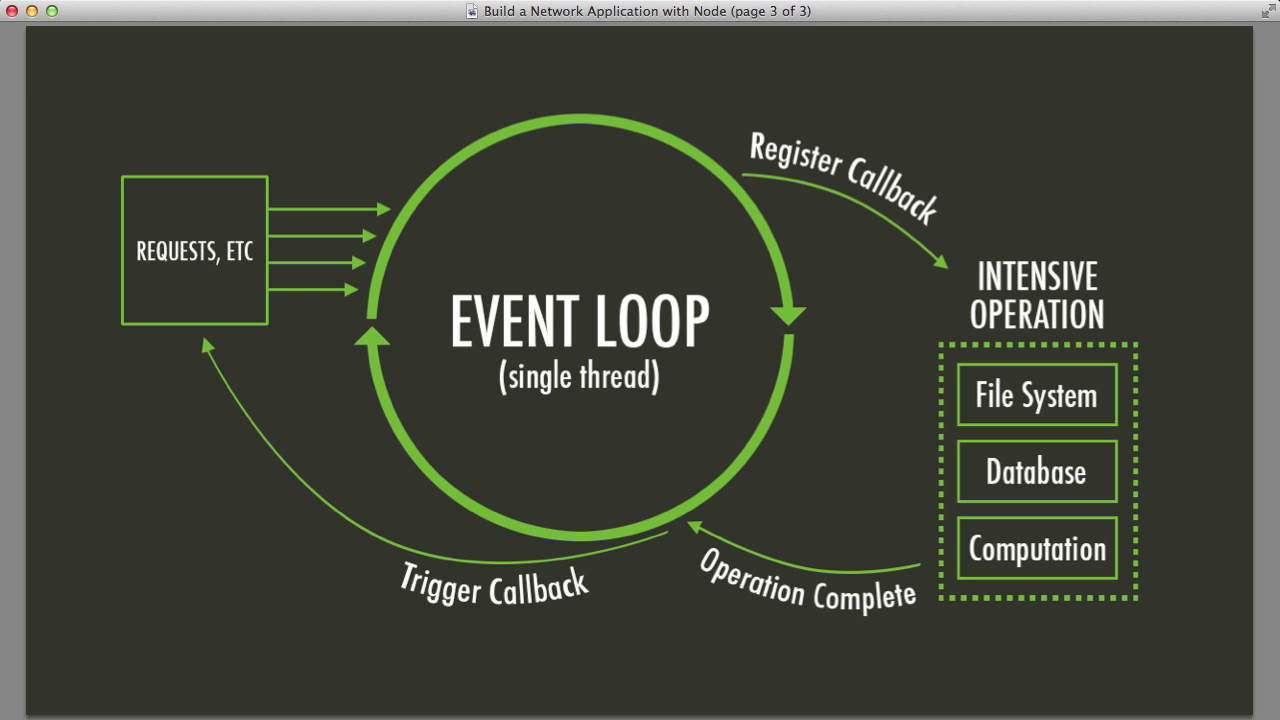
\includegraphics[width=6cm]{Clases/img/modelo_js.png}
            \caption{Modelo de JavaScript, node.js}
            \label{}
        \end{figure}
    
    \item Se crea una capacidad de poder ``atender mientras que esperan que algo pase'', JS funcionaba así, se polpularizó con Node.js. 
        \begin{enumerate}
            \item Se volvió en un tread que se le delegó el nombre de ``event loop sigle thread''.
            \item Podía procesar varios requests al mismo tiempo por que tenía una sistema similar a el de una ``sala de espera'', en lo que me daba mi resultado me daba un ``callback'' y atendía al siguiente request.
            \item Consideración: si se computaba algo muy complicado se trababa el tread.
        \end{enumerate}
    
    
    \item Modelo a detalle:
        \begin{figure}[htbp]
            \centering
            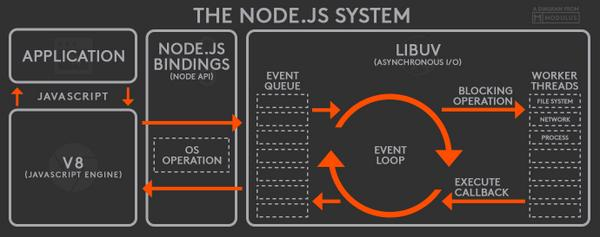
\includegraphics[width=6cm]{Clases/img/modelo_node.jpg}
            \caption{Modelo de node a detalle (aún más simplificado a comparación de lo que realmente pasa detrás de cámaras)}
            \label{}
        \end{figure} 
         
\end{enumerate}

%%%%%%%%%%%%%%%%%%%%%%%%%%%%%%%%%%%%%%%%%%%%%%%%%%%%%%%%%%%%%%%%%%%%%%%%%%%%%%%%%%%%%%%%%%%%%%%%
\section{Razones para usar node.js}
\begin{enumerate}
    \item Short turnaround / fast prototyping, 
        \begin{itemize}
            \item \emph{\textbf{Ejemplo: }Cada vez que se quería prototipar en un cambio se tardaba muchísimo en compilar y en correr que programador en c++, java; JavaScript soluciona eso ya que permite ver y porbar casi inmediatamente, es un lenguaje rápido.}
        \end{itemize}
    \item JavaScript Affordability:    
        \begin{itemize}
            \item No se necesita linux, permite po ejemplo escribir una función en JS y subirla a algun cloud service que cobra por ejecución de la función.
        \end{itemize}
    
    \item Time to market is faster:
        \begin{itemize}
            \item Se pueden utilizar lamba functions, subirlo al cloud es algo que rápidamente se prueba, ejecuta, y empezar a venderse en el mercado rápidamente.
        \end{itemize}
\end{enumerate}

%%%%%%%%%%%%%%%%%%%%%%%%%%%%%%%%%%%%%%%%%%%%%%%%%%%%%%%%%%%%%%%%%%%%%%%%%%%%%%%%%%%%%%%%%%%%%%%%
\section{Problemas con node.js \& JavaScript}
\begin{enumerate}
    \item Cada cosita es un paquete:
        \begin{itemize}
            \item No es como python que tiene una gran librería es super dependiente:
            \begin{figure}[htbp]
                \centering
                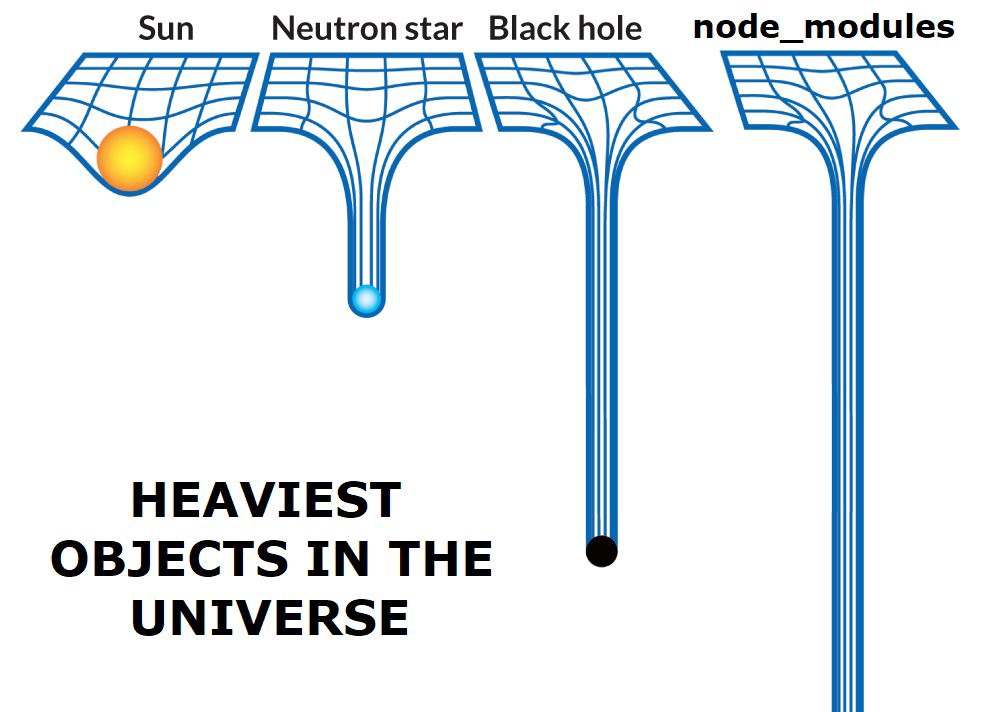
\includegraphics[width=6cm,angle=90]{Clases/img/heavy_node_js.jpeg}
                \caption{Meme de qué tan pesado son las librerías}
                \label{}
            \end{figure} 
        
        \item El asunto es que la librerías que tenían dependencias y que node.js dependía de ellas, rápidamente se podía acumular hasta un gigabyte en librerías. Esto daba lugar a otras inconmutabilidades ya que hay librerías que son co-dependientes y cuando se actualiza alguna puede ser que se arruine otra librería que dependa de la librería actualizada.
        \item \emph{\textbf{Observación: }Mala práctica de Docker no incluir los modules en los paquetes de Docker.}
        \item Se puede tardar un montón en instalar dependencias, usualmente media vez se corra una vaz el .log lo guarda en cache.
        \end{itemize}
    
    \item Utiliza mucho RAM:
        \begin{itemize}
            \item V8 no estaba optimizado en absoluto para uso de RAM, V8 va intentar usar toda la Ram
            \item Esto eventualmente se vuelve insostenible, este problema de memoria viene desde las épocas antiguas de C, a muchas personas se les olvidaba desocupar la memoria y lo mismo pasaba con node (denominados ``memory leak''), en node es muy complicado encontrar ``memory leaks'', el garbage colector tiene límites.
            \item \emph{\textbf{Recordar lo siguiente: }Affordability, si se utiliza algo mucho pesado en términos de pesado, es mejor no considerar node.js y mejor usar go, .net, c\#.}
        \end{itemize}
    
    \item Slow maths: 
        \begin{itemize}
            \item Si se intenta computar algo muy es muy lento, JavaScript es pésimo para matemática, JavaScript tiene un tipo de dato de número ``number'' custom made, adicionalmente es inconsistente con los floats.
            \item JavaScript nunca contempló esto por que se hizo a la carrera, pero si uno tiene operaciónes que hacer operaciones ``sincronas'' no use JavaScript.
            \item \textbf{Nos preguntamos:} ¿si tengo una compu de cuatro cores JavaScript va a usarlos todos o solo uno? Solo va a usar un core, por que el event loop es de \textbf{un sigle thread}, para operaciónes síncronas.
            \item \emph{\textbf{Observación: }Es así por asuntos de simplificad y de seguridad por eso es ineficiente con operaciones matemáticas.}
        \end{itemize}
\end{enumerate}

%%%%%%%%%%%%%%%%%%%%%%%%%%%%%%%%%%%%%%%%%%%%%%%%%%%%%%%%%%%%%%%%%%%%%%%%%%%%%%%%%%%%%%%%%%%%%%%%
\section{\textbf{Nos preguntamos:} ¿Hay que usar node.js?}
\begin{enumerate}
    \item Sí, apréndalo y evalúe que necesita su aplicación, porque node.js no es bueno para todo hay evaluar si sería una mejor opción usar go, etc.
    \item \textbf{Nos preguntamos:} ¿Node.js será la solución del futuro?
        \begin{itemize}
            \item No exactamente pero se va a seguir usando por lo menos para los siguientes 10 años.  
        \end{itemize}
\end{enumerate}

%%%%%%%%%%%%%%%%%%%%%%%%%%%%%%%%%%%%%%%%%%%%%%%%%%%%%%%%%%%%%%%%%%%%%%%%%%%%%%%%%%%%%%%%%%%%%%%%
\section{Cómo aprender node.js}
\begin{enumerate}
    \item Encontrar algo que quiera hacer e intentar hacerlo en node.js.
\end{enumerate}

%%%%%%%%%%%%%%%%%%%%%%%%%%%%%%%%%%%%%%%%%%%%%%%%%%%%%%%%%%%%%%%%%%%%%%%%%%%%%%%%%%%%%%%%%%%%%%%%
\section{Consideraciones}
\begin{enumerate}
    \item Ver: REDIS
    \item Proyecto próximo se desarrollará en python o node.js.
\end{enumerate}
